\chapter{Loop Closure}
\label{chapter:loop_closure}

Dieses Kapitel beschäftigt sich mit der Detektion von Schleifenschlüssen und der damit verbundenen Optimierung der initialen Schätzung einer Trajektorie beziehungsweise eines Pose-Graphen, entlang dessen ein Sensorsystem bewegt wurde. Im Folgenden wird zunächst näher auf den Detektionsschritt eingegangen. Auf Basis dessen wird in den drauf folgenden Abschnitten die in dieser Arbeit verwendete Methode zur Optimierung des Pose-Graphen eruiert.

\section{Detektion}

Dieser Abschnitt befasst sich mit der Detektion von Schleifenschlüssen in einem Pose-Graphen. Die hier vorgestellte Methode kann sowohl in einem inkrementell erweiterten Pose-Grahen, zum Beispiel als zusätzlicher Schritt in einem SLAM Verfahren, als auch in einem Nachbearbeitungsschritt auf einen bereits fertigen Graphen angewandt werden. Die Methode und die Optimierung des Graphen ist dabei zunächst vollständig losgelöst von der TSDF-Karte, die im Anschluss optimiert wird. Mehr dazu in Kapitel \ref{chapter:map_update}. Die vorliegenden initiale Schätzung der Roboter-Trajektorie kann das Ergebnis eines inkrementellen SLAM Ansatzes sein oder lediglich auf Odometrie-Schätzung beruhen.

Bevor nach Schleifenschlüssen gesucht werden kann, gilt es zu bestimmen, von welcher Pose aus gesucht werden soll. In einem inkrementellen SLAM Verfahren wäre das jeweils die aktuell betrachtete, zuletzt in den Graphen eingefügte Pose. In einem Nachbearbeitungsschritt wird dieser inkrementelle Prozess imitiert, indem der Pose-Graph, beginnend von der ersten eingefügten Pose, abgelaufen wird. In beiden Fällen wird also ein Schleifenschluss mit Posen gesucht, die früher in den Graphen eingefügt wurden als die aktuelle Pose $P_{cur}$. In einem ersten Schritt wird hierzu eine Menge von Schleifenschluss-Kandidaten erstellt. Diese Menge ergibt sich aus der in \cite{borrmann2008globally, shan2020lio} vorgestellten euklidischen Distanzmetrik, die in dieser Arbeit verwendet wird. Eine Pose $P_i$ gilt als Schleifenschluss-Kandidat zu $P_{cur}$, wenn die euklidische Distanz zwischen den beiden Posen geringer ist als eine parametrisierbare Schwelle $d_{max}$. Zusätzlich zu diesem Parameter wird an dieser Stelle ein weiterer Parameter $d_{trav}$ eingeführt der die minimale Distanz definiert, die der Sensorsystem entlang des Teilpfades gegeben durch $P_i$ und $P_{cur}$ zurückgelegt hat. Um Posen zu identifizieren, die diese Voraussetzungen Erfüllen, wird ein \textbf{k-d tree (k-d Baum)} \cite{bentley1975multidimensional} verwendet. Ein k-d Baum ist eine Datenstruktur zur Speicherung von (räumlichen) Informationen, die durch assoziative Suchen abgefragt werden können. Ein k-d Baum eignet sich aufgrund der optimierten Laufzeit besonders für räumliche Suchen. Dabei steht das \textbf{k} für die Dimensionalität des Suchraums \cite{bentley1975multidimensional}. An dieser Stelle wird der k-d Baum zur Speicherung von \textbf{3-d} Daten genutzt. Diese ergeben sich aus den Posen des Pfades. Vor jeder Detektion wird ein neuer k-d Baum aus den Translationsanteilen aller zuvor eingefügten Posen aufgebaut. Im Anschluss wird eine Radius-Suche durchgeführt, die alle Daten des k-d Baumes (hier 3-d Punkte) zurückliefert, deren euklidische Distanz zu einer übergebenen Position geringer ist als eine übergebene Schwelle. Die übergebene Position ist dabei der Translationsanteil von $P_cur$ und die übergebene Schwelle $d_max$. Ergebnis ist eine Menge von Kandidaten für Schleifenschlüsse $\mathbb{K} = \left\lbrace K_0, ..., K_k \right\rbrace$. Diese Arbeit verwendet die k-d Baum Implementation der \textbf{Pointcloud Library (PCL)} \ref{rusu20113d}.

Über die generierten Kandidaten ist an dieser Stelle lediglich bekannt, dass sie sich im nicht optimierten Pfad in der Nähe der aktuellen Pose $P_{cur}$ befinden. Diese räumliche Nähe ist an dieser Stelle allerdings nur eine Annahme, die es zu verifizieren gilt. Als Basis für die Verifikation dient die in diesem Ansatz gegebene Datenbasis in Form von zu jeder Pose des Pose-Graphen $\mathfrak{P}_{init} = \left\lbrace P_0, ..., _n \right\rbrace$ zugehörigen Punktwolken $ \mathbb{C} = \left\lbrace C_0, ..., C_n \right\rbrace$. Für die aktuell betrachte Pose $P_{cur}$ und die zugehörige Punktwolke wird ein Scan-Matching gegen jeden Kandidaten aus  $\mathbb{K}$ und dessen zugehörigen Punktwolken $C_i$ durchgeführt und evaluiert. Konvergiert das Scan-Matching mit einer festgelegten Genauigkeit ist der Kandidat validiert. Im Folgenden wird die Punktwolke der aktuell betrachteten Pose $P_{cur}$ als Scan-Punktwolke $C_{scan}$ und die zum zu validierenden Kandidaten zugehörige Punktwolke als Model-Punktwolke $C_{model}$ bezeichnet. Grundlage für das Scan-Matching der beiden Punktwolken ist ein Algorithmus wie \textbf{ICP}, \textbf{GICP} oder vergleichbare Algorithmen zur Registrierung von Punktwolken. Diese Algorithmen liefern neben einer Information zur Konvergenz in der Regel zusätzlich ein Maß dafür zurück, wie gut die Punktwolken nach der Registrierung aufeinander passen. In dieser Arbeit werden hierzu die Implementationen der Algorithmen der Pointcloud Library \cite{rusu20113d} verwendet. Diese liefern für beide Algorithmen einen \textbf{Fitness-Score ($\Gamma$)} zurück, der die durchschnittliche quadrierte Distanz zwischen einem Punkt der Scan-Punktwolke und dem euklidisch nächste Punkt der Model-Punktwolke nach Registrierung der Scan-Punktwolke an die Model-Punktwolke beschreibt. Nachfolgende Formel zeigt diesen Sachverhalt mit $s_i$ als aktuellen Scanpunkt und $m_i$ als zugehörigen, euklidisch nächsten Punkt der Model-Punktwolke und $N$ als Anzahl der Punkte in der Scan-Punktwolke.

\begin{myequation}
\Gamma = \frac{\sum_{i = 0}^{N} \norm{\vec{m_i} - \vec{s_i}}^2}{N}
\end{myequation}

Liegt der Fitness-Score unter eine vordefinierten Schwelle $\Gamma_{max}$, ist der Kandidat validiert.
Zusätzlich liefern die Algorithmen die bestimmte finale Transformation $T_{fin}$ der Registrierung von Scan zu Model. Da GICP und ICP deutlich bessere Ergebnisse erzielen, wenn zwischen den Daten bereits eine Initialschätzung vorliegt, wird eine solche, auf Basis der jeweiligen Pose-Differenzen, genutzt. Die Punktwolkendaten liegen hier jeweils relativ zur Pose, von derer sie aufgenommen wurden, vor. Für die Initialschätzung wird nun die Model-Punktwolke ins Koordinatensystem der Scan-Punktwolke transformiert. Dazu wird zunächst die Transformation $T_{model \rightarrow scan}$ über die zugehörigen Posen $P_{model}$ und $P_{scan}$ und die zugehörigen Transformationen $T_{model \rightarrow map}$ und $T_{scan \rightarrow map}$ von den Posen ins Ursprungskoordinatensystem bestimmt:

\begin{myequation}
T_{model \rightarrow scan} = T_{scan \rightarrow map}^{-1} \cdot T_{model \rightarrow map}
\end{myequation}

Im Anschluss wird jeder Punkt $p_{model}^i$ der Punktwolke $C_{model}$ mit der bestimmten Transformation $T_{model \rightarrow scan}$ transformiert. Nun ist die Model-Punktwolke in das Koordinatensystem der Scan-Punktwolke, gegeben die aktuellen Pose-Schätzungen, vortransformiert. Diese Vortransformation muss nach der anschließenden Registrierung mittels ICP, GICP oder einem ähnlichen Verfahren für die Berechnung der finalen Transformation berücksichtigt werden. Dies ist in Abbildung \ref{fig:LoopIdentifikation} dargestellt. Sie führt zusätzlich die vom zur Registrierung berechneten Algorithmus bestimmte Transformation $T_{reg}$, sowie die sich daraus ergebene neue, approximative Pose $P_{scan}'$, von der die Scan-Punktwolke aufgenommen wurde. Die finale Transformation $T_{scan' \rightarrow model}$ die im weiteren Verlauf für die Optimierung des Pose-Graphen benötigt wird ergibt sich wie folgt:

\begin{myequation}
\label{math:final_transformation}
T_{scan' \rightarrow model} = T_{model \rightarrow scan}^{-1} \cdot T_{reg}
\end{myequation}

\begin{figure}
		\centering
		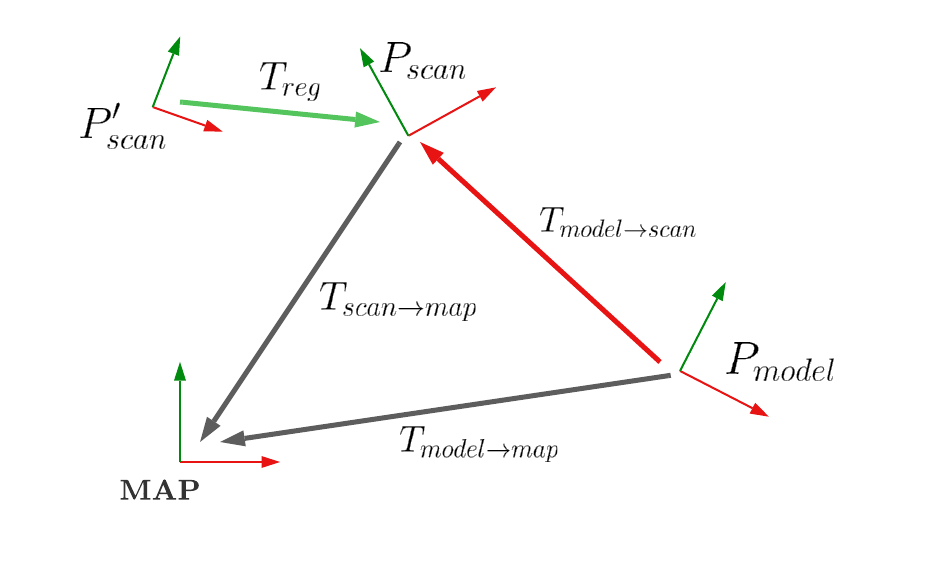
\includegraphics
			[scale=0.3]
			{LoopIdentifikation}
		\caption
			[Caption for LOF]{Diese Grafik stellt die Posen und Transformationen dar, die bei der Detektion eines Schleifenschlusses zur Verwendung kommen. Dabei bestimmt $T_{model \rightarrow scan}$ die Vortransformation vom lokalen Model-Koordinatensystem in das des Scans (dargestellt in rot). In grün dargestellt ist die Transformation $T_reg$, die von dem verwendeten Algorithmus zur Registrierung der Scan-Punktwolke an die mit $T_{model \rightarrow scan}$ vortransformierte Model-Punktwolke, ausgegeben wird. Eine Kombination der Transformationen $T_reg$ und $T_{model \rightarrow scan}$ ergibt die finale, zur Optimierung des Pose-Graphen verwendete Transformationen. Diese Kombination ist in Gleichung \ref{math:final_transformation} definiert.}		                                                                                                                                     
		\label{fig:LoopIdentifikation}
\end{figure}

Auf diese Art und Weise können nur wenige Schleifenschlüsse identifiziert werden. Ursache ist zu diesem Zeitpunkt das Scan-Matching, welches zwar in den meisten Fällen konvergiert, jedoch fast keinen der Kandidaten aufgrund zu hoher Fitness-Scores validieren kann. Zusätzlich sind einige der identifizierten Schleifenschlüsse, besonders in Bereichen von Fluren oder Orten mit wenigen Features, fehlerhaft. Hier sind zwar die genannten Rahmenbedingungen erfüllt, allerdings verschlechtern die Schleifenschlüsse das Ergebnis maßgeblich. Um diese Problem zu lösen wurden mehrere Ansätze implementiert und evaluiert. Dazu wurde zunächst das Problem des Scan-Matching näher betrachtet. Dabei stellt sich heraus, dass für ein gute Transformations-Schätzung der Scan-Matching Algorithmen neben einer guten Initial-Schätzung zusätzlich eine dichtere Model-Punktwolke essentiell ist. Basierend auf der Annahme, dass eine lokale Umgebung $\left\lbrace P_{i - x}, ..., P_i, ..., P_{i+x} \right\rbrace$ um eine Pose $P_i$ konsistent registriert ist, wurde die Model-Punktwolke um die Punktwolken aus der direkten Nachbarschaft, gegeben durch den Parameter $x$, angereichert. Dazu wird jeweils die Pose-Differenz zur Model-Punktwolke berechnet und die Punktwolke entsprechend der berechneten Transformation ins Koordinatensystem der Model-Punktwolke angereichert. Ergebnis ist eine deutlich dichtere Punktwolke, was die Korrespondenzfindung für die Scan-Matching Algorithmen deutlich verbessert und so zu einem besseren Endergebnis führt. Abbildung \ref{fig:Windows} zeigt die durchschnittlichen Fitness-Scores aller Schleifenschluss-Kandidaten der jeweiligen Iteration für ein durch $x$ gegebenes Fenster um die Model-Punktwolke herum.

%\begin{figure}
%		\centering
%		\includegraphics
%			[scale=0.8]
%			{Windows_small}
%		\caption
%			[Caption for LOF]{Diese Grafik zeigt den Einfluss des Fensters für die Anreicherung der Model-Punktwolke bei der Validierung gefundener Schleifenschluss-Kandidaten, gegeben die Größe des Fensters $x$. Rote vertikale Linien markieren Posen, an den Schleifenschlüsse detektiert und aufgrund des geringen Fitness-Scores validiert wurden. Die Gesamtmenge der Posen, deren Punktwolken zu einer dichteren Model-Punktwolke zusammengeführt werden, beträgt $2 \cot x + 1$. Es ist zu erkennen, dass der durchschnittlich berechnete Fitness-Score mit steigendem $x$ im Schnitt niedriger ist. Allerdings wird die Verringerung ab einem gewissen Punkt unwesentlich. Hier sind zwischen einer Wahl von $x = 2$ bis $x = 6$ nur geringe Unterschiede zu erkennen. Die Größten Veränderungen sind zwischen $x = 0$ und $x = 2$ zu erkennen. Hier sinkt der durchschnittliche Fitness-Score merklich. Dies trifft auch auf die Ergebnisse im Scan-Matching zu. Diese verbessern sich bei zunehmendem $x$, hier sind ebenfalls die größten Veränderungen zwischen $x=0$ und $x=2$ zu sehen. Die Wahl des Fenster korreliert zusätzlich mit dem durchschnittlichen absoluten Fehler zwischen der durch die Schleifenschlüsse optimierten Trajektorie eines Datensatz und der zugehörigen \textbf{Ground-Truth}. }	                                                                                                                                     
%		\label{fig:Windows}
%\end{figure}

\begin{figure}
	\centering
	\begin{subfigure}{.5\textwidth}
		 \centering
  		 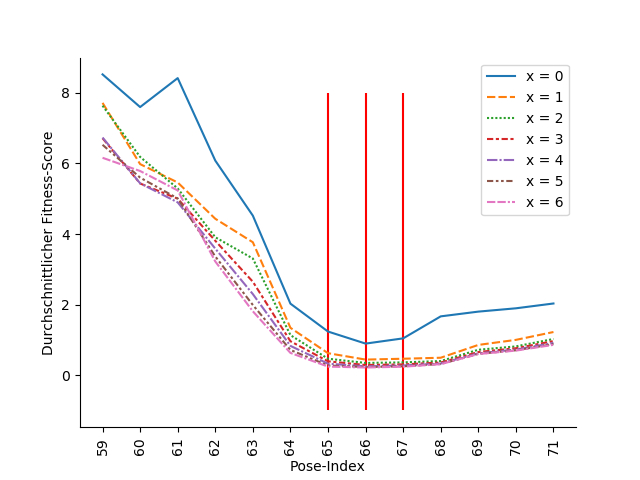
\includegraphics[width=.95\linewidth]{Windows_small}
  		 \centering \caption{Durchschnittlicher Fitness-Score für gefundene Schleifenschluss-Kandidaten eines Datensatz von Pose $0$ bis Pose $80$, Posen ohne Kandidaten sind nicht dargestellt.}
  		 \label{fig:single_tsdf}
	\end{subfigure}%
	\begin{subfigure}{.5\textwidth}
    	\centering
  		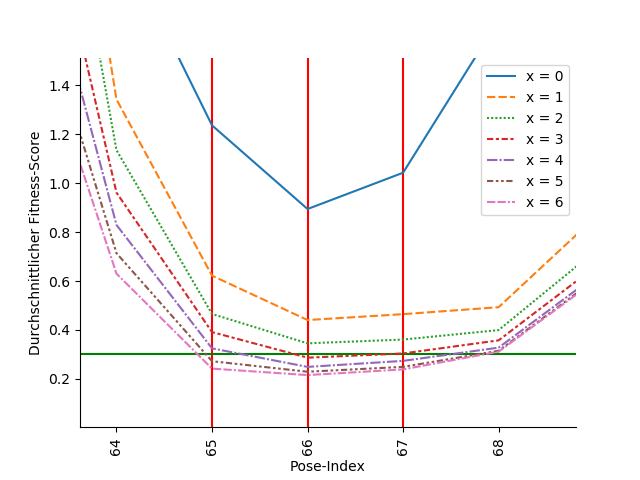
\includegraphics[width=.95\linewidth]{Windows_small_limit}
  		\centering \caption{Vergrößerung des Bereiches von links, in dem Schleifenschlüsse gefunden und validiert wurden. Dargestellt als grüne horizontale Linie ist die parametrisierte Schranke für Schleifenschlüsse.}
  		\label{fig:approx_cloud}
	\end{subfigure}
	\caption{Diese Grafik zeigt den Einfluss des Fensters für die Anreicherung der Model-Punktwolke bei der Validierung gefundener Schleifenschluss-Kandidaten, gegeben die Größe des Fensters $x$. Rote vertikale Linien markieren Posen, an den Schleifenschlüsse detektiert und aufgrund des geringen Fitness-Scores validiert wurden. Die Gesamtmenge der Posen, deren Punktwolken zu einer dichteren Model-Punktwolke zusammengeführt werden, beträgt $2 \cdot x + 1$. Es ist zu erkennen, dass der durchschnittlich berechnete Fitness-Score mit steigendem $x$ im Schnitt niedriger ist. Allerdings wird die Verringerung ab einem gewissen Punkt unwesentlich. Hier sind zwischen einer Wahl von $x = 2$ bis $x = 6$ nur geringe Unterschiede zu erkennen. Die Größten Veränderungen sind zwischen $x = 0$ und $x = 2$ zu erkennen. Hier sinkt der durchschnittliche Fitness-Score merklich. Dies trifft auch auf die Ergebnisse im Scan-Matching zu. Diese verbessern sich bei zunehmendem $x$, hier sind ebenfalls die größten Veränderungen zwischen $x=0$ und $x=2$ zu sehen. Die Wahl des Fenster korreliert zusätzlich mit dem durchschnittlichen absoluten Fehler zwischen der durch die Schleifenschlüsse optimierten Trajektorie eines Datensatz und der zugehörigen \textbf{Ground-Truth}.}
	\label{fig:Windows}
\end{figure}

Ein weiteres, bereits angeschnittenes Problem sind Schleifenschlüsse, die zwar die vorgegebenen Rahmenbedingungen erfüllen, allerdings grundsätzlich fehlerhaft sind. Hier ist zum Beispiel in einem Flur das Scan-Matching aufgrund einer sehr Feature armen Umgebung konvergiert und die Validierung auf Basis des Fitness-Scores konnte zusätzlich keinen Fehler bei der Registrierung identifizieren. Dann werden häufig Positionen, die in einer initialen Schätzung weit auseinander liegen aufeinander gezogen. Zusätzlich kann es vorkommen, dass das Scan-Matching mit einem guten Fitness-Score konvergiert, obwohl die Umgebungen nicht zueinander passen. Die berechnete finale Transformation ist in diesem Fall so fehlerhaft, dass sie nicht mit der initialen Schätzung vereinbar ist. Aus diesem Grund wurden zwei Validatoren beziehungsweise \textbf{Rejector} entwickelt, die neben dem Fitness-Score zusätzliche Validations-Stufen einführen. Dies ist zum einen der \textbf{Linien-Rejector} und auf  der anderen Seite der \textbf{Reichweiten-Rejector}. Diese nutzen die Unsicherheiten der einzelnen Posen aus. Vor Beginn das Algorithmus erfolgt eine Einschätzung über die Sicherheit der initial bestimmten Posen. Diese kann beliebig schlecht gewählt werden um sicherzustellen, dass bei der Optimierung gewünschte Änderungen vorgenommen werden. Dies erhöht allerdings die Wahrscheinlichkeit für fehlerhafte Schleifenschlüsse, die durch die beiden im Folgenden beschriebenen Validatoren nicht erfasst werden können. Kann für eine Initial-Schätzung zum Beispiel aufgrund voriger Erfahrungen ein gewisser Fehler für die Translation und Rotation zwischen aufeinander folgenden Posen abgeschätzt werden, sollte dieser im Folgenden verwendet werden.

\textbf{\textsl{Linien-Rejector}}

Je nach Parametrisierung ist es möglich, dass Schleifenschlüsse zwischen Posen $P_{cur}$ und $P_{prev}$ identifiziert werden, deren Zwischen-Posen näherungsweise auf einer Linie liegen. Der maximale Abstand einer Zwischen-Pose zur durch $P_{cur}$ und $P_{prev}$ definierten Linie ist mit $d_{line}$ definiert und parametrisierbar. Standardmäßig ist $d_{line} = 0.5m$. Eine beschriebene Identifikation ist im Regelfall möglich, wenn, wenn $d_{max} > d_{trav}$. In Ausnahmefällen kann dies bei bestimmten Trajektorien schon für geringere $d_{trav}$ der Fall sein. Diese Art von Schleifenschlüssen stellt im Grundsatz kein Problem dar, allerdings ist es durch die Bewertung des Ergebnisses des Scan-Matching anhand des Fitness-Scores besonders in Fluren oder ähnlichen Regionen, die unvorteilhaft für ein Scan-Matching sind, möglich, dass am Schleifenschluss beteiligte Posen ohne Rücksicht auf die initialen Schätzungen und Zwischen-Posen aufeinander gezogen werden. Abbildung \ref{Line-Rejector} zeigt dieses dies schematisch und nimmt zusätzlich Bezug auf die Identifikation von diesen besonderen Fällen.

\begin{figure}
		\centering
		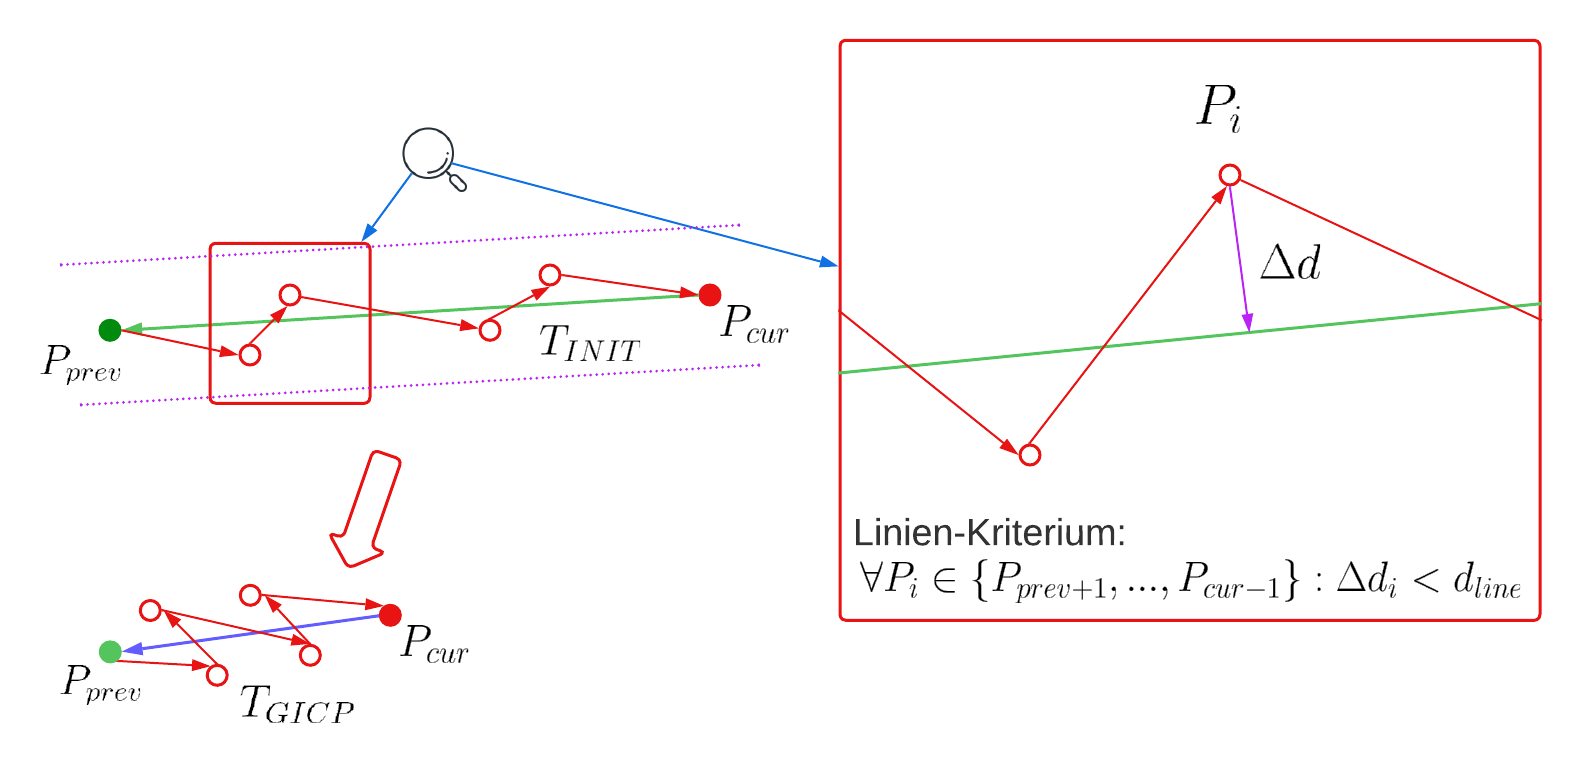
\includegraphics
			[scale=0.27]
			{Line-Rejector}
		\caption
			[Caption for LOF]{Diese Grafik beschreibt die Funktionsweise des Linien-Rejectors. Zusätzlich definiert sie das mathematische Kriterium für eine approximative Linie, gegeben $d_{line}$: $\forall P_i \in \left\lbrace P_{prev + 1}, ..., P_{cur - 1} \right\rbrace : \Delta d_i < d_{line}$. Die Abbildung ist zweigeteilt. In der rechten Vergrößerung eines Teilbereichs der oben links dargestellten Trajektorie ist das Linien-Kriterium dargestellt. Die Linie zwischen den beiden Posen $P_{cur}$ und $P_{prev}$ ist oben links und in der Vergrößerung in grün dargestellt. Sie wird durch den Translationsanteil von $T_{init}$, der initial gegebenen Transformation zwischen $P_{cur}$ und $P_{prev}$, sowie den Translationsanteil von $P_{cur}$ als Stützvektor gegeben. Durch lila gestrichelte Linien ist die Umgebung dargestellt, in der sich das Sensorsystem befindet. In diesem Fall handelt es sich um einen besonders Feature-armen Flur. Bei der Validierung mittels Scan-Matching (in diesem Fall per GICP) wurde die durch $T_{GICP}$ beschriebene Transformation ermittelt. In diesem Fall ist das Scan-Matching mit einem sehr guten Fitness-Score konvergiert, obwohl die Transformation Augenscheinlich fehlerhaft ist. Dies liegt an der beschriebenen Umgebung, die aus Sicht des Laserscanners für verschiedene Posen sehr ähnlich, wenn nicht nahezu identisch aussieht. Dies sind sehr schlechte Voraussetzungen für ein Scan-Matching. Unten links ist die zu erwartende Optimierung der Trajektorie auf Basis der fehlerhaften Transformation $T_{GICP}$. Bei den Zwischen-Posen tritt durch die Stauchung der Geraden ein Ziehharmonika-Effekt auf. Dies hat fatale Auswirkungen auf die generierte Karte und den weiteren Verlauf der Trajektorie.}                                                                                                                                     
		\label{fig:Line-Rejector}
\end{figure}

Wie bereits zuvor beschrieben, ist eine mögliche Lösung dieses Problems die Ausnutzung von relativen, lokalen Unsicherheiten zwischen aufeinanderfolgenden Posen. Der Linien-Rejector nutzt dabei die definierten Unsicherheiten für die Translation als Vektor aus den gegebenen Standardabweichungen: $\vec{\sigma_t} = \left(\sigma_x, \sigma_y, \sigma_z \right)$. Diese können entweder konstant gegeben oder für jede Pose-Differenz aufeinander folgender Posen einzeln, zum Beispiel anhand von Berechnungen im SLAM Ansatz, gegeben sein. Im Folgenden werden die Standardabweichungen als konstant angenommen. Gegeben $P_{cur}$ und $P_{prev}$, die Anzahl an Zwischen-Posen $N_{between}$, sowie die konstante Standardabweichung der Translation $\vec{\sigma_t}$ lässt sich nun Konfidenzintervall berechnen, in dem basierend auf der gegebenen Standardabweichung ein gewisser Prozentsatz der für $P_{cur}$ möglichen liegt. Dies ist in 3D ein räumlicher Bereich. Als Erwartungswert wird die initiale Schätzung für $P_{cur}$, genauer gesagt dessen Translationsanteil $\vec{t_{cur}}$ verwendet. Damit ergibt sich für die untere Grenze $\vec{t_u}$ und obere Grenze $\vec{t_o}$ des Konfidenzintervalls unter Ausnutzung der akkumulierten Standardabweichungen zwischen $P_{prev}$ und $P_{cur}$:

\begin{myequation}
\vec{t_u} = \vec{t_{cur}} - \left( N_{between} + 1 \right) \cdot k \cdot \vec{\sigma_t}
\end{myequation}

\begin{myequation}
\vec{t_o} = \vec{t_{cur}} + \left( N_{between} + 1 \right) \cdot k \cdot \vec{\sigma_t}
\end{myequation}

Dabei bezeichnet $k$ die verwendete standardisierte Intervallgrenze. Im Folgenden wird hierfür $1$ verwendet, eine beliebige Anpassung dieses Wertes ist möglich. Für $k=1$ werden für eine gegebene Standardabweichung im Konfidenzintervall etwa $80\%$ bis $85\%$ der möglichen relativen Pose-Änderungen zwischen aufeinander folgenden Posen abgedeckt. Der Prozentsatz des durch $\vec{t_u}$ und $\vec{t_o}$ abgedeckten Volumens berechnet sich aus folgender Potenz:

\begin{myequation}
\prod_{i=0}^{N_{between}} 0.8
\end{myequation}

Zugrunde liegt die Schätzung des Prozentsatzes, der durch die Intervallgrenzen, gegeben $k$ abgedeckt wird (hier etwa $80\%$). Für $4$ Zwischen-Posen beträgt die Abdeckung in diesem Fall in etwa $33\%$. Für eine größere Abdeckung ist ein größeres $k$ zu wählen. Mit zunehmender Anzahl an Zwischen-Posen wird der durch den Rejector abgedeckte Bereich verhältnismäßig immer kleiner, obwohl er linear vergrößert wird. Dies hat eine sehr strenge Behandlung von Schleifenschlüssen auf Linien zur Folge. Mit einem größeren $k$ kann dies entschärft werden. Liegt $P_{cur}$ nach Bestimmung der neuen Transformation $T_{GICP}$ außerhalb des durch $\vec{t_u}$ und $\vec{t_o}$ beschriebenen Volumens, der gefundene Schleifenschluss als ungültig angesehen. Liegt die neue Pose innerhalb des Volumens, ist sie validiert. Auf diese Weise konnten in einem Beispieldurchlauf für eine Fenster-Größe von $x = 0$ und $\Delta d = 2.0m$ bei einem Datensatz mit $200$ Posen $8$ fehlerhafte Schleifenschlüsse identifiziert und verworfen werden. Mit größerer Fenstergröße reduziert sich die Anzahl dieser fehlerhaften Schleifenschlüsse. So konnten bereits bei einer Größe von $x = 2$ in diesem Datensatz keine fehlerhaften Schleifenschlüsse identifiziert werden. Diese sind jedoch auch weiterhin nicht ausgeschlossen, weshalb der Rejector als weitere Sicherheitsschranke hinter das Scan-Matching geschaltet wird.

\textbf{\textsl{Reichweiten-Rejector}}

Der \textbf{Reichweiten-Rejector} basiert auf dem identischen Prinzip wie der zuvor erläuterte Linien-Rejector. Hier wird zusätzlich zur Standardabweichung in der Translation auch die Standardabweichung in der Rotation berücksichtigt. Zusätzlich ist das Vorhandensein einer Linie keine Voraussetzung für diesen Rejector. Alle anderen mathematischen Verhältnisse aus dem oben vorgestellten Rejector treffen so auch hier zu und werden analog sowohl für die Translation, als auch für die Rotation angewandt.  Dieser Rejector greift ist dem Linien-Rejector nachgeschaltet.

Der nachfolgende Abschnitt beschäftigt sich mit der Optimierung des Pose-Graphen auf Basis identifizierter Schleifenschlüsse.

\section{Graphenoptimierung}



Bezug zu GTSAM Library Beschreibung aufnehmen.
Wichtigste verwendete Funktionen bennen.
Verweis auf GTSAM Paper.
Erklärung von Faktorgraphen und Faktoren.
Erklärung der Genutzten datenstrukturen und optimizer.
Erklärung von noise constraints (Unsicherheiten)

\section{Optimierungen}

1. Vorregistrierung

2. Filtern der Punktwolke

3. Unterschiedliche Scan-Matching Varianten
	1. ICP
	2. GICP
	3. Kurz auf Teaser++ eingehen
	4. VGICP
	
	-> Analyse des Scan Matchings bezogen auf 1. Vorregistrierung, 2. LC Detektion Matching
	-> Graph über Fitness Counter mit LC Linie (dünn) verschiedene Farben
	-> dazu: starten mit allen varianten und jeweils werte akkumulieren
	-> schreiben in csv
	
	4. Rejectors
	
	\improvement{einführen: Pointcloud-Enrichment, Grafik: Fitness score im bezug zum enrichment: eine wolke vs. mehrere}

\section{Pseudocode}


\improvement{insert the pseudo code to the whole algorithm}
	
\section{Datensätze}

Verwendete Datensätze und herausforderungen herausstellen

\subsection{Hannover1}

Herausforderungen:

- Datensatz allgemein: falsches Koordindatensystem -> Transformation beschreiben

- extrem fehlerbehaftete Rotation in zweitem Kreis (Lösung: Vorregistrierung ICP)
(Scan-Matching bekommt extrem divergierte Wolken nicht mehr aufeinander)

- problematisch: fehlerhafte LC Optimierung durch schlechtes Scan Matching (Grund: Feature-armer Flur) -> mögliche ( noch zu entwickelnde) Lösung: LC's auf Linien gesondert betrachten -> Identifikation eines LC auf Linien -> Betrachtung der Scan Matching Transformation - wenn aufGeraden kann die Transformation die beiden LC-Punkte nicht vollständig zusammen ziehen

\subsection{Maps}

\section{Evaluation}


